\documentclass[aspectratio=169,12pt]{beamer}
\usepackage[utf8]{inputenc}
\usepackage{amsmath, amssymb}
\usepackage{booktabs}
\usepackage{colortbl}
\usepackage{hyperref}
\usepackage{makecell}
\usepackage{ragged2e}
\usepackage{bytefield}
\usepackage{tikz}
\usetikzlibrary{arrows.meta, positioning, shapes.geometric, calc, tikzmark, shapes.misc}
\usetheme{Madrid}

\title{Computer Structure}
\subtitle{System}
\author{Lihu Rappoport}
\date{}

\begin{document}

\frame{\titlepage}


\begin{frame}{Basic DRAM chip}
\begin{itemize}
\item The DRAM memory is implemented as a 2-dimensional array of cells
\begin{itemize}
\item Arranged in rows and columns
\end{itemize}
\end{itemize}

\begin{center}
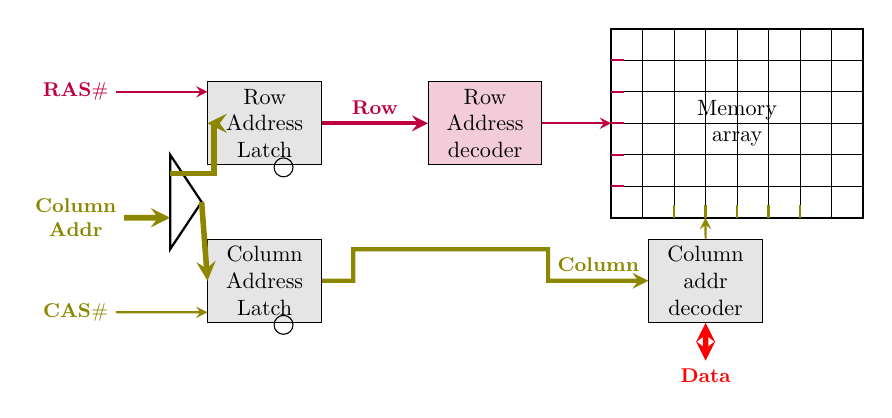
\begin{tikzpicture}[scale=0.8, transform shape,
    block/.style={draw, fill=gray!20, minimum width=1.8cm, minimum height=1cm, align=center},
    decoder/.style={draw, fill=purple!20, minimum width=1.8cm, minimum height=1.2cm, align=center},
    signal/.style={->, >=stealth, thick},
    label/.style={font=\small\bfseries}
]

% Row Address Latch
\node[block, text width=1.5cm] (rowlatch) at (0,0) {Row Address Latch};

% Column Address Latch
\node[block, text width=1.5cm] (collatch) at (0,-2.5) {Column Address Latch};

% Row Address decoder
\node[decoder, text width=1.5cm] (rowdecoder) at (3.5,0) {Row Address decoder};

% Column decoder
\node[block, text width=1.5cm] (coldecoder) at (7,-2.5) {Column addr decoder};

% Memory array - draw as grid
\draw[thick] (5.5,1.5) rectangle (9.5,-1.5);
\foreach \x in {6,6.5,7,7.5,8,8.5,9} {
    \draw (\x,1.5) -- (\x,-1.5);
}
\foreach \y in {1,0.5,0,-0.5,-1} {
    \draw (5.5,\y) -- (9.5,\y);
}
\node[align=center] at (7.5,0) {Memory\\array};

% Input signals
\node[label, purple] (ras) at (-3,0.5) {RAS$\#$};
\draw[signal, purple] (ras) -- (rowlatch.west|-ras);

\node[label, olive] (cas) at (-3,-3) {CAS$\#$};
\draw[signal, olive] (cas) -- (collatch.west|-cas);

\node[label, olive, align=center] (addr) at (-3,-1.5) {Column\\Addr};
\draw[signal, olive, line width=2pt] (addr) -- (-1.5,-1.5);

% Multiplexer symbol
\draw[thick] (-1.5,-0.5) -- (-1.5,-2) -- (-1,-1.25) -- cycle;
\draw[signal, olive, line width=2pt] (-1,-1.25) -- (collatch.west);
\draw[signal, olive, line width=2pt] (-1.5,-0.8) -- (-0.8,-0.8) -- (-0.8,0) -- (rowlatch.west);

% Connections between blocks
\draw[signal, purple, line width=1.5pt] (rowlatch.east) -- node[above, font=\small\bfseries, purple] {Row} (rowdecoder.west);
\draw[signal, olive, line width=1.5pt] (collatch.east) -- ++(0.5,0) -- ++(0,0.5) -- (4.5,-2) -- (4.5,-2.5) -- node[above, font=\small\bfseries, olive] {Column} (coldecoder.west);

% Row decoder to memory array
\draw[signal, purple] (rowdecoder.east) -- (5.5,0);
% Draw wordlines
\foreach \y in {1,0.5,0,-0.5,-1} {
    \draw[purple, thick] (5.5,\y) -- (5.7,\y);
}

% Column decoder to memory array
\draw[signal, olive] (coldecoder.north) -- (7,-1.5);
% Draw bitlines
\foreach \x in {6.5,7,7.5,8,8.5} {
    \draw[olive, thick] (\x,-1.5) -- (\x,-1.3);
}

% Data I/O
\node[label, red] (data) at (7,-4) {Data};
\draw[signal, red, line width=2pt, <->] (data) -- (coldecoder.south);

% Clock symbols
\draw (0.3,-0.7) circle (0.15);
\draw (0.3,-3.2) circle (0.15);

\end{tikzpicture}
\end{center}

\begin{itemize}
\item DRAM access sequence
\begin{itemize}
\item Put Row address on the address bus
\item Assert RAS$\#$ (Row Address Strobe) to latch the selected Row
\item Put Column address on the address bus
\item Wait RAS$\#$ to CAS$\#$ delay and assert CAS$\#$ (Column Address Strobe) to latch the Column
\item Get data on address bus after CL (CAS latency)
\end{itemize}
\end{itemize}

\end{frame}
\end{document}